\thispagestyle{hoccungpinone}
\pagestyle{hoccungpi}
\everymath{\color{hoccungpi}}
\graphicspath{{../hoccungpi/pic/}}
\blfootnote{\color{hoccungpi}\color{hoccungpi}$^1$Giáo viên Toán tại trường Don Bosco, thành phố Nice, Cộng Hòa Pháp.}
\begingroup
\AddToShipoutPicture*{\put(0,616){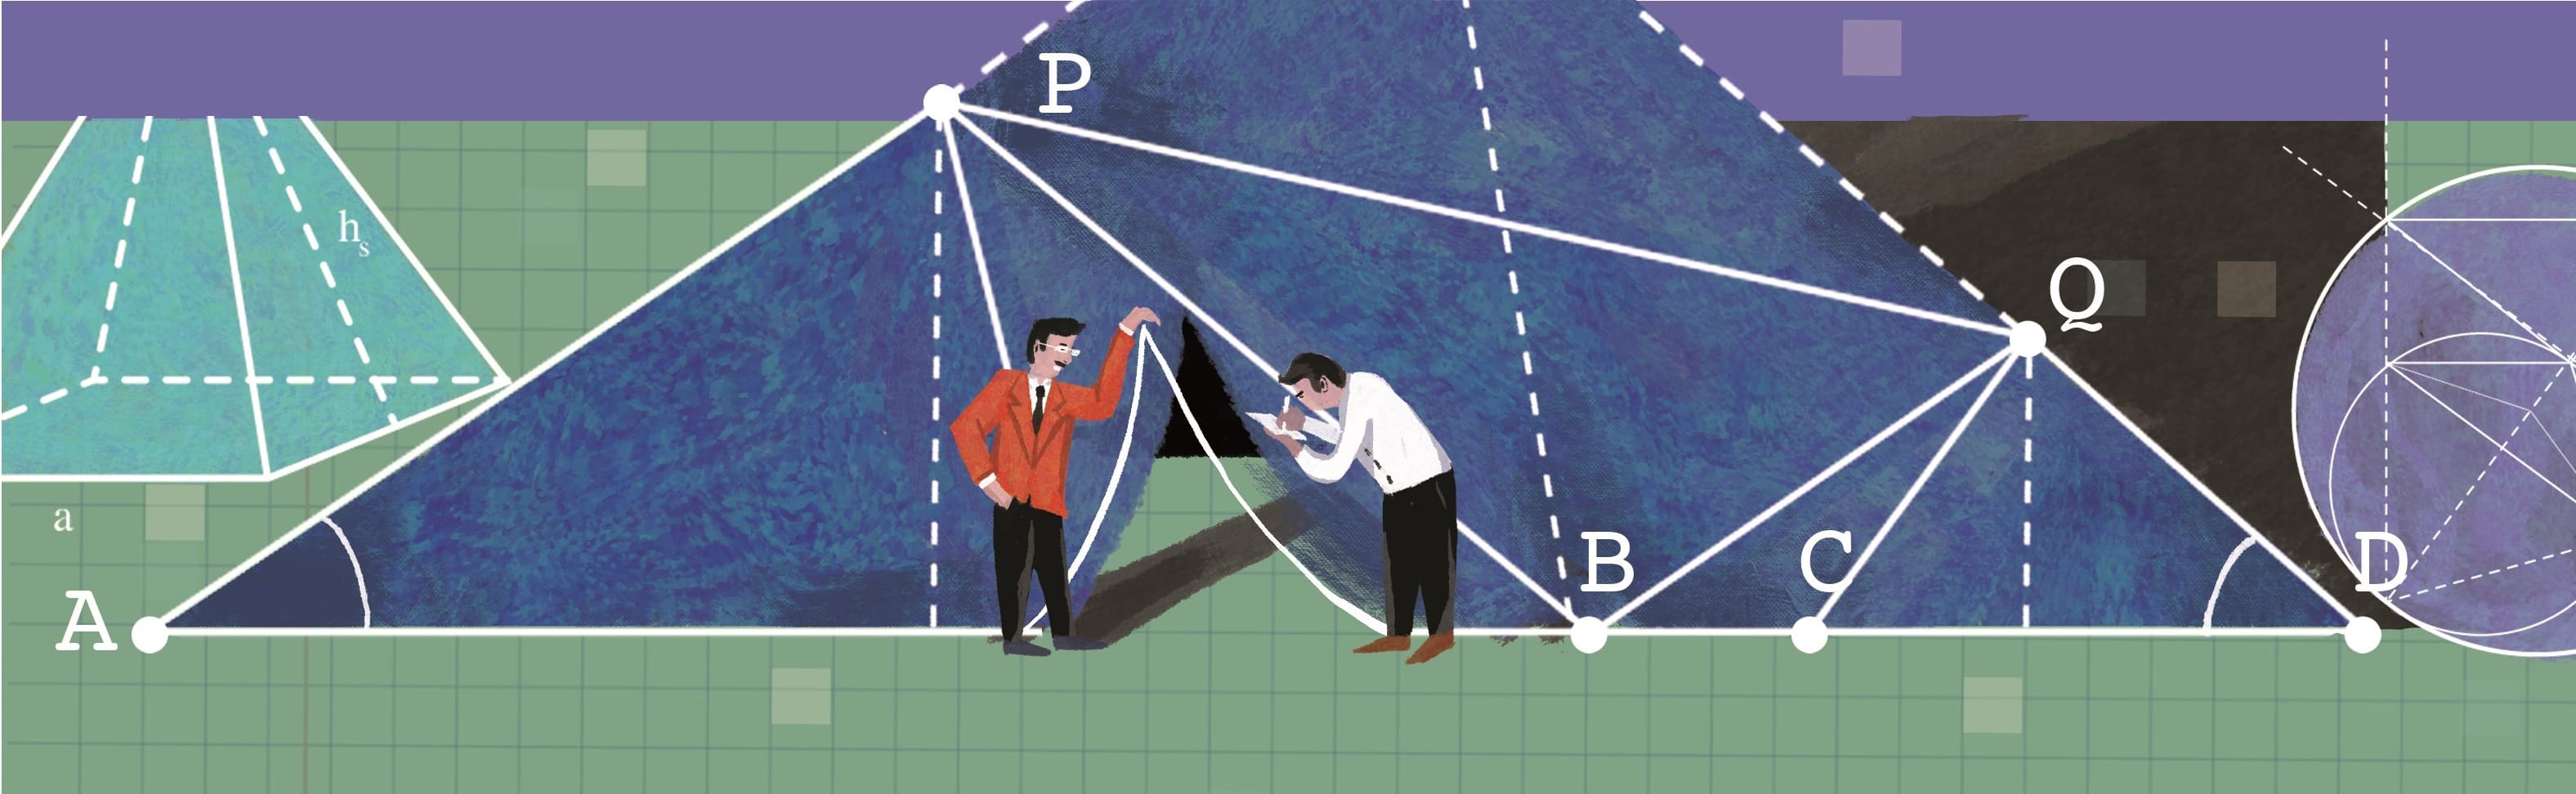
\includegraphics[width=19.3cm]{../bannerhoccungpi}}}
\AddToShipoutPicture*{\put(114,525){
\includegraphics[scale=1]{../tieude.pdf}}}
\centering
\endgroup
\vspace*{180pt}

\begin{multicols}{2}
	\textbf{\color{hoccungpi}Vài nét chung về thuật toán Dijkstra.}
	\vskip 0.1cm
	Lý thuyết đồ thị là một nhánh của Toán học và của Tin học nhằm mô hình hóa những vấn đề khác nhau thường gặp trong cuộc sống bởi những đồ thị. Một trong những vấn đề cổ điển của lý thuyết đồ thị là mô hình hóa mạng lưới đường bộ giữa các thành phố (làng, xã \ldots), đặc biệt hơn một trong những bài toán đặt ra là tối ưu hóa khoảng cách, thời gian di chuyển cũng như giá thành di chuyển từ thành phố này tới thành phố khác. Cụ thể hơn là tìm con đường tốt nhất về khía cạnh khoảng cách, thời gian, giá thành \!\ldots\,\! để di chuyển từ thành phố này tới thành phố khác. Việc tìm con đường tốt nhất nhắc tới trong bài toán tổng quát nêu trên được đưa về việc tìm con đường ngắn nhất nối hai đỉnh tương ứng trên một đồ thị.
	\vskip 0.1cm
	Để dễ hình dung, ta xét một mạng lưới đường bộ biểu diễn như hình dưới đây được trích dẫn từ Wikipedia.
	\vskip 0.1cm
	Một mạng lưới như thế được gọi là một đồ thị. Ở đây những thành phố từ $A$ tới $J$ được gọi là các đỉnh của đồ thị. Các thành phố đó được nối với nhau bởi những con đường mà ta gọi là các cạnh của đồ thị. Mỗi cạnh được gán với một giá trị mà ta gọi là trọng số của cạnh. Trọng số trong ví dụ này biểu diễn khoảng cách được đo bằng đơn vị km giữa hai thành phố liên kết với nhau. Bài toán đặt ra là tìm đường đi ngắn nhất từ thành phố $A$ tới thành phố $J$. 
	\begin{figure}[H]
		\vspace*{-5pt}
		\centering
		\captionsetup{labelformat= empty, justification=centering}
		\begin{tikzpicture}[hoccungpi,scale=0.8]
			\draw  (0.26,4.18)-- (2.78,5.02);
			\draw  (2.78,5.02)-- (2.86,3.8);
			\draw  (2.86,3.8)-- (2.,2.76);
			\draw  (2.86,3.8)-- (4.02,2.42);
			\draw  (4.02,2.42)-- (4.74,3.4);
			\draw  (4.02,2.42)-- (4.,0.);
			\draw  (4.,0.)-- (6.8,3.36);
			\draw  (6.8,3.36)-- (2.78,5.02);
			\draw  (0.26,4.18)-- (0.26,2.46);
			\draw  (0.26,2.46)-- (1.54,1.);
			\draw  (1.54,1.)-- (4.,0.);
			\begin{scriptsize}
				\draw [fill=hoccungpi] (2.86,3.8) circle (8pt) node {$\color{white}C$};
				\draw [fill=hoccungpi] (2.,2.76) circle (8pt) node {$\color{white}G$};
				\draw [fill=hoccungpi] (4.02,2.42) circle (8pt) node {$\color{white}H$};
				\draw [fill=hoccungpi] (4.74,3.4) circle (8pt) node {$\color{white}D$};
				\draw [fill=hoccungpi] (2.78,5.02) circle (8pt) node {$\color{white}A$};
				\draw [fill=hoccungpi] (0.26,4.18) circle (8pt) node {$\color{white}B$};
				\draw [fill=hoccungpi] (0.26,2.46) circle (8pt) node {$\color{white}F$};
				\draw [fill=hoccungpi] (1.54,1.) circle (8pt) node {$\color{white}I$};
				\draw [fill=hoccungpi] (4.,0.) circle (8pt) node {$\color{white}J$};
				\draw [fill=hoccungpi] (6.8,3.36) circle (8pt) node {$\color{white}E$};
				\draw (1.46,4.9) node {$85$};
				\draw (2.56,4.3) node {$217$};
				\draw (2.2,3.4) node {$186$};
				\draw (3.1,3.05) node {$103$};
				\draw (4.68,2.7) node {$183$};
				\draw (3.74,1.39) node {$167$};
				\draw (5.7,1.65) node {$502$};
				\draw (4.96,4.4) node {$173$};
				\draw (0.,3.49) node {$80$};
				\draw (0.55,1.69) node {$250$};
				\draw (2.58,0.3) node {$84$};
			\end{scriptsize}
		\end{tikzpicture}
		\vspace*{-10pt}
	\end{figure} 
	Ta xét một ví dụ khác về mạng lưới tàu hỏa của một thành phố như đồ thị dưới đây.
	\begin{figure}[H]
		\vspace*{-5pt}
		\centering
		\captionsetup{labelformat= empty, justification=centering}
		\begin{tikzpicture}[hoccungpi,scale=0.7]
			\draw  (0.,3.)-- (1.5,4.78);
			\draw  (1.5,4.78)-- (2.14,1.18);
			\draw  (0.,3.)-- (2.14,1.18);
			\draw  (2.14,1.18)-- (4.08,2.76);
			\draw  (6.24,5.)-- (4.08,2.76);
			\draw  (4.08,2.76)-- (1.5,4.78);
			\draw  (1.5,4.78)-- (6.24,5.);
			\draw  (6.24,5.)-- (8.58,3.42);
			\draw  (8.58,3.42)-- (7.,1.);
			\draw  (7.,1.)-- (4.08,2.76);
			\draw  (4.08,2.76)-- (8.58,3.42);
			\draw  (7.,1.)-- (6.24,5.);
			\draw  (2.14,1.18)-- (7.,1.);
			\draw [fill=hoccungpi] (0.,3.) circle (1.5pt);
			\draw (-0.3,3.17) node {$A$};
			\draw [fill=hoccungpi] (1.5,4.78) circle (1.5pt);
			\draw (1.64,5.15) node {$B$};
			\draw [fill=hoccungpi] (2.14,1.18) circle (1.5pt);
			\draw (2.04,0.89) node {$C$};
			\draw [fill=hoccungpi] (4.08,2.76) circle (1.5pt);
			\draw (4.06,3.33) node {$D$};
			\draw [fill=hoccungpi] (6.24,5.) circle (1.5pt);
			\draw (6.38,5.37) node {$E$};
			\draw [fill=hoccungpi] (7.,1.) circle (1.5pt);
			\draw (7.2,0.77) node {$F$};
			\draw [fill=hoccungpi] (8.58,3.42) circle (1.5pt);
			\draw (8.72,3.79) node {$G$};
			\begin{scriptsize}
				\draw (1.04,3.87) node {$4$};
				\draw (1.56,3.11) node {$7$};
				\draw (0.88,2.03) node {$8$};
				\draw (3.36,1.91) node {$10$};
				\draw (4.98,4.29) node {$15$};
				\draw (3.,4.07) node {$18$};
				\draw (3.94,5.39) node {$21$};
				\draw (7.54,4.49) node {$17$};
				\draw (7.96,2.11) node {$7$};
				\draw (5.16,1.83) node {$12$};
				\draw (5.6,3.43) node {$31$};
				\draw (6.74,4.03) node {$10$};
				\draw (4.6,0.85) node {$25$};
			\end{scriptsize}
		\end{tikzpicture}
		\vspace*{-10pt}
	\end{figure}
	Ở đây các đỉnh từ $A$ tới $G$ của đồ thị đại diện cho các ga tàu. Mỗi cạnh của đồ thị thể hiện rằng có đường tàu nối giữa hai ga. Trọng số trên mỗi cạnh chính là thời gian di chuyển tính bằng phút từ ga này tới ga kia. Bài toán đặt ra là làm thế nào tìm đường đi nhanh nhất để di chuyển từ ga $B$ tới ga $G$. 
	\vskip 0.1cm
	Để giải quyết những bài toán như trên, vào năm $1959$, nhà Toán học đồng thời là nhà Khoa học máy tính người Hà Lan, E.W. Dijkstra ($1930 - 2022$) đã đề xuất một thuật toán cho phép tính toán đường đi ngắn nhất giữa một đỉnh cụ thể và tất cả các đỉnh khác trong một đồ thị mà ở đó tất cả các trọng đó đều dương. Thuật toán bắt đầu từ việc gán trọng số bằng $0$ cho đỉnh xuất phát và bằng vô cùng cho các đỉnh còn lại. Quá trình xử lý của thuật toán bao gồm kiểm tra lần lượt các đỉnh, chọn ra đỉnh có khoảng cách nhỏ nhất tính từ đỉnh xuất phát và cập nhật trọng số cho các đỉnh lân cận của đỉnh được chọn. Tiếp tục quá trình xử lý trên cho tới khi đỉnh kết thúc được chọn hoặc cho tới khi không còn đỉnh để chọn thì dừng lại. Ta thu được đường đi ngắn nhất.
	\vskip 0.1cm
	\textbf{\color{hoccungpi}Thuật toán Dijkstra dưới dạng bảng.}
	\vskip 0.1cm 
	Để hiểu hơn về thuật toán Dijkstra, trong mục này ta tập trung vào giải một trong hai bài toán nêu ở mục trước.
	\vskip 0.1cm
	\textbf{\color{hoccungpi}Bài toán:} Tìm đường đi ngắn nhất nối hai thành phố là hai đỉnh $A$ và $J$ của đồ thị cho bởi hình bên. Trọng số trên các cạnh thể hiện khoảng cách tính bằng km từ thành phố này tới thành phố kia. 	
	\begin{figure}[H]
		\vspace*{-5pt}
		\centering
		\captionsetup{labelformat= empty, justification=centering}
		\vspace*{-5pt}\begin{tikzpicture}[hoccungpi,scale=0.8]
			\draw  (0.26,4.18)-- (2.78,5.02);
			\draw  (2.78,5.02)-- (2.86,3.8);
			\draw  (2.86,3.8)-- (2.,2.76);
			\draw  (2.86,3.8)-- (4.02,2.42);
			\draw  (4.02,2.42)-- (4.74,3.4);
			\draw  (4.02,2.42)-- (4.,0.);
			\draw  (4.,0.)-- (6.8,3.36);
			\draw  (6.8,3.36)-- (2.78,5.02);
			\draw  (0.26,4.18)-- (0.26,2.46);
			\draw  (0.26,2.46)-- (1.54,1.);
			\draw  (1.54,1.)-- (4.,0.);
			\begin{scriptsize}
				\draw [fill=hoccungpi] (2.86,3.8) circle (8pt) node {$\color{white}C$};
				\draw [fill=hoccungpi] (2.,2.76) circle (8pt) node {$\color{white}G$};
				\draw [fill=hoccungpi] (4.02,2.42) circle (8pt) node {$\color{white}H$};
				\draw [fill=hoccungpi] (4.74,3.4) circle (8pt) node {$\color{white}D$};
				\draw [fill=hoccungpi] (2.78,5.02) circle (8pt) node {$\color{white}A$};
				\draw [fill=hoccungpi] (0.26,4.18) circle (8pt) node {$\color{white}B$};
				\draw [fill=hoccungpi] (0.26,2.46) circle (8pt) node {$\color{white}F$};
				\draw [fill=hoccungpi] (1.54,1.) circle (8pt) node {$\color{white}I$};
				\draw [fill=hoccungpi] (4.,0.) circle (8pt) node {$\color{white}J$};
				\draw [fill=hoccungpi] (6.8,3.36) circle (8pt) node {$\color{white}E$};
				\draw (1.46,4.9) node {$85$};
				\draw (2.56,4.3) node {$217$};
				\draw (2.2,3.4) node {$186$};
				\draw (3.1,3.05) node {$103$};
				\draw (4.68,2.7) node {$183$};
				\draw (3.74,1.39) node {$167$};
				\draw (5.7,1.65) node {$502$};
				\draw (4.96,4.4) node {$173$};
				\draw (0.,3.49) node {$80$};
				\draw (0.55,1.69) node {$250$};
				\draw (2.58,0.3) node {$84$};
			\end{scriptsize}
		\end{tikzpicture}
		\vspace*{-10pt}
	\end{figure}
	Thuật toán Dijkstra được tiến hành như sau.
	\vskip 0.1cm
	\textit{Bước $1$: Khởi đầu.} Ta dựng một bảng gồm các cột là những đỉnh của đồ thị như hình dưới đây. Vì ta xuất phát từ đỉnh $A$ nên ta gán trọng số là $0$ và các đỉnh còn lại có trọng số là vô cùng. Ta ghi $0_A$ trong cột chứa đỉnh $A$ và vô cùng trong những cột còn lại. Điều này có nghĩa là ở bước $1$, xuất phát từ $A$ ta có thể đi tới $A$ mất $0$ km và ta chưa đi tới những đỉnh khác. 
	\begin{table}[H]
		\vspace*{-5pt}
		\centering
		\captionsetup{labelformat= empty, justification=centering}
		\resizebox{\columnwidth}{!}{\begin{tabular}{|c|c|c|c|c|c|c|c|c|c|c|}
				\hline
				Đỉnh được chọn&$A$&	$B$&	$C$&	$D$&	$E$&	$F$&	$G$&	$H$&	$I$&	$J$\\
				\hline
				Xuất phát&	$0_A$&	$\infty$&	$\infty$&	$\infty$&	$\infty$&	$\infty$&	$\infty$&	$\infty$&	$\infty$&	$\infty$\\
				\hline
		\end{tabular}}
		%		\caption{\small\textit{\color{}.}}
		\vspace*{-10pt}
	\end{table}
	\textit{Bước $2$: Chọn đỉnh đầu tiên và cập nhật trọng số cho các đỉnh còn lại.}   
	Ta chọn giá trị nhỏ nhất ở dòng cuối cùng trong bảng vẽ ở bước $1$. Ở đây giá trị nhỏ nhất là $0_A$ tương ướng với đường đi từ $A$ tới chính nó với khoảng cách là $0$~km.
	\vskip 0.1cm
	$\bullet$ Đóng khung giá trị nhỏ nhất được chọn. 
	\vskip 0.1cm
	$\bullet$ Trong cột Đỉnh được chọn ta ghi đỉnh được chọn cũng như khoảng cách tương ứng. Ở đây ta ghi $A(0)$.
	\vskip 0.1cm
	$\bullet$ Ta xóa tất cả các ô nằm ngay phía dưới ô được đóng khung. Điều này có nghĩa là xuất phát từ $A$ ta đã tìm ra đường đi ngắn nhất tới $A$ và không cần tìm thêm những đường đi khác nữa.
	\vskip 0.1cm 
	Dựa vào đồ thị ta thấy rằng, từ đỉnh $A$ ta có thể di chuyển tới các đỉnh $B$, $C$ và $E$ với các khoảng cách tương ứng là $85$ km, $217$ km và $173$ km. So với những trọng số vô cùng đã gán ở bước $1$, ta thấy rằng những giá trị mới nhỏ hơn, nên ở dòng thứ $3$ của bảng, tương ứng với các đỉnh $B$, $C$ và $E$, ta ghi $85_A$, $217_A$ và $173_A$ thay vì những giá trị vô cùng. Những đỉnh còn lại vẫn giữ nguyên giá trị được gán ở bước $1$. Chỉ số $A$ ở dưới những giá trị muốn nói rằng ta di chuyển từ đỉnh $A$.
	\vskip 0.1cm 
	Ta có bảng mới như sau: 
	\begin{table}[H]
		\vspace*{-5pt}
		\centering
		\captionsetup{labelformat= empty, justification=centering}
		\resizebox{\columnwidth}{!}{\begin{tabular}{|c|c|c|c|c|c|c|c|c|c|c|}
				\hline
				Đỉnh được chọn&$A$&	$B$&	$C$&	$D$&	$E$&	$F$&	$G$&	$H$&	$I$&	$J$\\
				\hline
				Xuất phát&	$[0_A ]$	&$\infty$&	$\infty$&	$\infty$	&$\infty$	&$\infty$&	$\infty$&	$\infty$&	$\infty$	&$\infty$\\
				\hline
				$A(0)$&		&$85_A$	&$217_A$&	$\infty$	&$173_A$&	$\infty$&	$\infty$&	$\infty$&	$\infty$&	$\infty$\\
				\hline
		\end{tabular}}
		\vspace*{-10pt}
	\end{table}
	\textit{Bước $3$: Chọn đỉnh thứ hai và cập nhật trọng số cho các đỉnh còn lại.}  Ta chọn trọng số nhỏ nhất ở dòng cuối cùng trong bảng vẽ ở bước $2$. Ở đây giá trị nhỏ nhất là $85_A$ tương ướng với đường đi từ $A$ tới đỉnh $B$ với khoảng cách là  $85$ km.
	\vskip 0.1cm
	$\bullet$ Đóng khung giá trị nhỏ nhất được chọn. 
	\vskip 0.1cm
	$\bullet$ Trong cột Đỉnh được chọn ta ghi đỉnh được chọn cũng như khoảng cách tương ứng. Ở đây đỉnh được chọn là đỉnh $B$ nên ta ghi $B(85)$.
	\vskip 0.1cm
	Ta xóa tất cả các ô nằm ngay phía dưới ô được đóng khung. Điều này có nghĩa là xuất phát từ $A$ ta đã tìm ra đường đi ngắn nhất tới $B$ và không cần tìm thêm những đường đi khác nữa. 
	\vskip 0.1cm
	Từ đỉnh $B$ ta chỉ có thể di chuyển tới đỉnh $F$ với khoảng cách tương ứng là $80$ km. Ta tính được khoảng cách nhỏ nhất từ $A$ tới $F$ là $85+80=165$ km. So với trọng số đã gán trước đó cho đỉnh $F$ ta chọn giá trị nhỏ hơn, nên ở dòng thứ $4$ của bảng, đỉnh $F$ được gán giá trị mới là $165_B$, các đỉnh còn lại vẫn giữ nguyên giá trị. Ta hiểu $165_B$ ở đây chính là tổng khoảng cách nhỏ nhất từ $A$ tới $B$ và từ $B$ tới $F$.
	\vskip 0.1cm 
	Ta được bảng mới như sau: 
	\begin{table}[H]
		\vspace*{-5pt}
		\centering
		\captionsetup{labelformat= empty, justification=centering}
		\resizebox{\columnwidth}{!}{\begin{tabular}{|c|c|c|c|c|c|c|c|c|c|c|}
				\hline
				Đỉnh được chọn&$A$&	$B$&	$C$&	$D$&	$E$&	$F$&	$G$&	$H$&	$I$&	$J$\\
				\hline
				Xuất phát&	$[0_A ]$	&$\infty$&	$\infty$&	$\infty$	&$\infty$	&$\infty$&	$\infty$&	$\infty$&	$\infty$	&$\infty$\\
				\hline
				$A(0)$&		&$85_A$	&$217_A$&	$\infty$	&$173_A$&	$\infty$&	$\infty$&	$\infty$&	$\infty$&	$\infty$\\
				\hline
				$B(85)$	&	&	&$217_A$&	$\infty$&	$173_A$&	$165_B$&	$\infty$	&$\infty$&	$\infty$	&$\infty$\\
				\hline
		\end{tabular}}
		\vspace*{-10pt}
	\end{table}
	\textit{Bước $4$: Chọn đỉnh thứ ba và cập nhật trọng số cho các đỉnh còn lại.}  Lặp lại bước $3$ với dòng cuối cùng của bảng trên ta thu được đỉnh thứ ba cần chọn là đỉnh $F$ vì có trọng số nhỏ nhất. Từ đỉnh $F$ ta chỉ có thể di chuyển tới đỉnh $I$ với khoảng cách tương ứng là $250$ km. Ta tính được khoảng cách nhỏ nhất từ $A$ tới $I$ là $165+250=415$ km. So với trọng số đã gán trước đó cho đỉnh $I$ ta chọn giá trị nhỏ hơn, nên ở dòng thứ $5$ của bảng, đỉnh $I$ được gán giá trị mới là $415_F$, các đỉnh còn lại vẫn giữ nguyên giá trị. 
	\vskip 0.1cm
	Ta được bảng mới như sau: 
	\begin{table}[H]
		\vspace*{-5pt}
		\centering
		\captionsetup{labelformat= empty, justification=centering}
		\resizebox{\columnwidth}{!}{\begin{tabular}{|c|c|c|c|c|c|c|c|c|c|c|}
				\hline
				Đỉnh được chọn&$A$&	$B$&	$C$&	$D$&	$E$&	$F$&	$G$&	$H$&	$I$&	$J$\\
				\hline
				Xuất phát&	$[0_A ]$	&$\infty$&	$\infty$&	$\infty$	&$\infty$	&$\infty$&	$\infty$&	$\infty$&	$\infty$	&$\infty$\\
				\hline
				$A(0)$&		&$85_A$	&$217_A$&	$\infty$	&$173_A$&	$\infty$&	$\infty$&	$\infty$&	$\infty$&	$\infty$\\
				\hline
				$B(85)$	&	&	&$217_A$&	$\infty$&	$173_A$&	$165_B$&	$\infty$	&$\infty$&	$\infty$	&$\infty$\\
				\hline
				$F(165)$&	&	&	$217_A$&	$\infty$	&$173_A$	&	&$\infty$&	$\infty$&	$415_F$	&$\infty$\\
				\hline
		\end{tabular}}
		\vspace*{-10pt}
	\end{table}
	\textit{Bước $5$ đến kết thúc: Lặp lại quá trình trên cho tới khi đỉnh kết thúc được chọn hoặc không còn đỉnh để chọn.}
	\vskip 0.1cm 
	$\bullet$ \textit{Dòng} $5$: Chọn đỉnh $E$, đóng khung trọng số $173_A$ và xóa tất cả các ô nằm dưới ô vừa được đóng khung. 
	\vskip 0.1cm
	$\bullet$ \textit{Dòng} $6$: Ghi $E(173)$ trong cột \textit{Đỉnh được chọn}. Cập nhật trọng số mới $675_E$ cho đỉnh $J$. Ở đây $675$ km chính là tổng khoảng cách từ $A$ tới $E$ và từ $E$ tới $J$. Các đỉnh còn lại vẫn giữ nguyên giá trị. Tiếp theo chọn đỉnh $C$, đóng khung trọng số $217_A$ và xóa tất cả các ô nằm dưới ô vừa được đóng khung.
	\vskip 0.1cm 
	$\bullet$ \textit{Dòng} $7$: Ghi $C(217)$ trong cột \textit{Đỉnh được chọn}. Từ đỉnh $C$ ta có thể di chuyển tới các đỉnh $G$ và $H$ với các khoảng cách tương ứng là $186$ km và $103$ km. Tổng khoảng cách ngắn nhất tương ứng tính từ $A$ tới các đỉnh $G$ và $H$ lần lượt là $217+186=403$ km và $217+103=320$ km. Ta cập nhật trọng số mới $403_C$ cho đỉnh $G$ và $320_C$ cho đỉnh $H$. Các đỉnh còn lại vẫn giữ nguyên. Tiếp theo chọn đỉnh $H$, đóng khung trọng số $320_C$ và xóa tất cả các ô nằm dưới ô vừa được đóng khung.
	\vskip 0.1cm
	$\bullet$ \textit{Dòng} $8$: Ghi $H(320)$ trong cột Đỉnh được chọn. Từ đỉnh $H$ ta có thể di chuyển tới các đỉnh $D$ và $J$ với các khoảng cách tương ứng là $183$ km và $167$ km. Tổng khoảng cách ngắn nhất tương ứng tính từ $A$ tới các đỉnh $D$ và $J$ lần lượt là $320+183=503$ km và $320+167=487$ km. Bằng cách chọn giá trị nhỏ nhất, ta cập nhật trọng số mới $503_H$ cho đỉnh $D$ và $487_H$ cho đỉnh $J$. Các đỉnh còn lại không thay đổi. Tiếp theo chọn đỉnh $G$, đóng khung trọng số $403_C$ và xóa tất cả các ô nằm dưới ô vừa được đóng khung.
	\vskip 0.1cm
	$\bullet$ \textit{Dòng} $9$: Ghi $G(403)$ trong cột \textit{Đỉnh được chọn}. Vì không có đường đi nào xuất phát từ $G$ tới những đỉnh còn lại (không tính những đỉnh đã bị loại), nên các giá trị của các đỉnh còn lại không thay đổi. Tiếp theo chọn đỉnh $I$, đóng khung trọng số $415_F$ và xóa tất cả các ô nằm dưới ô vừa được đóng khung. 
	\vskip 0.1cm
	$\bullet$ \textit{Dòng} $10$: Ghi $I(415)$ trong cột \textit{Đỉnh được chọn}. Trọng số của đỉnh $D$ không thay đổi vì không có đường đi từ $I$ tới $J$. Trọng số của đỉnh $J$ cũng vậy vì trọng số mới $415+84=499$ km lớn hơn trọng số ban đầu.  Chọn đỉnh $J$, đóng khung trọng số $487_H$ và xóa tất cả các ô nằm dưới ô vừa được đóng khung.
	\vskip 0.1cm 
	$\bullet$ \textit{Dòng $11$}: Ghi $J(487)$ trong cột \textit{Đỉnh được chọn}. Thuật toán kết thúc vì mục đích của ta là di chuyển từ $A$ tới $J$.  Ta được đường đi ngắn nhất có độ dài $487$ km. 
	\vskip 0.1cm
	Ta thu được bảng cuối cùng như sau:
	\begin{table}[H]
		\vspace*{-5pt}
		\centering
		\captionsetup{labelformat= empty, justification=centering}
		\resizebox{\columnwidth}{!}{\begin{tabular}{|c|c|c|c|c|c|c|c|c|c|c|}
				\hline
				Đỉnh được chọn&$A$&	$B$&	$C$&	$D$&	$E$&	$F$&	$G$&	$H$&	$I$&	$J$\\
				\hline
				Xuất phát&	$[0_A ]$	&$\infty$&	$\infty$&	$\infty$	&$\infty$	&$\infty$&	$\infty$&	$\infty$&	$\infty$	&$\infty$\\
				\hline
				$A(0)$&		&$85_A$	&$217_A$&	$\infty$	&$173_A$&	$\infty$&	$\infty$&	$\infty$&	$\infty$&	$\infty$\\
				\hline
				$B(85)$	&	&	&$217_A$&	$\infty$&	$173_A$&	$165_B$&	$\infty$	&$\infty$&	$\infty$	&$\infty$\\
				\hline
				$F(165)$&	&	&	$217_A$&	$\infty$	&$173_A$	&	&$\infty$&	$\infty$&	$415_F$	&$\infty$\\
				\hline
				$E(173)$	&	&	&$[217_A]$&	$\infty$&	&	&	$\infty$&	$\infty$&	$415_F$&	$675_E$\\
				\hline
				$C(217)$	&	&	&	&$\infty$&	&	&$403_C$&	$[320_C ]$&	$415_F$	&$675_E$\\
				\hline
				$H(320)$	&	&	&	&$503_H$&	&	&$[403_C]$&		&$415_F$&	$487_H$\\
				\hline
				$G(403)$&	&	&	&$503_H$&	&	&	&	&$[415_F ]$&	$487_H$\\
				\hline
				$I(415)$&	&	&	&$503_H$&	&	&	&	&	&$[487_H]$\\
				\hline
				$J(487)$&	&	&	& &	& & & & & \\
				\hline
		\end{tabular}}
		\vspace*{-10pt}
	\end{table} 		
	\textit{Bước $6$: Kết luận}. Dựa vào bảng trên ta kết luận rằng đường đi ngắn nhất xuất phát từ thành phố $A$ tới thành phố $J$ dài $487$ km. Để dựng lại con đường đó dựa vào bảng trên ta chỉ cần đọc các đỉnh theo chiều ngược lại từ $J$ tới $A$ như sau:
	\vskip 0.1cm
	$\bullet$ Xuất phát từ đỉnh $J$, ta đọc giá trị đóng khung là [$487_H$] , ta chọn chỉ số $H$ là đỉnh tiếp theo.
	\vskip 0.1cm
	$\bullet$ Ở cột chứa đỉnh $H$, giá trị đóng khung là [$320_C$], ta chọn $C$ là đỉnh tiếp theo.
	\vskip 0.1cm
	$\bullet$ Ở cột chứa đỉnh $C$, giá trị đóng khung là [$217_A$], ta chọn $A$ là đỉnh tiếp theo và cũng là đỉnh cuối cùng. 
	\vskip 0.1cm
	Đọc từ dưới lên trên, ta được đường đi ngắn nhất cần tìm là $A-C-H-J$ với khoảng cách ngắn nhất là $487$ km.
	\vskip 0.1cm 
	\textbf{\color{hoccungpi}Một số bài tập áp dụng.}
	\vskip 0.1cm 
	\textbf{\color{hoccungpi}Bài $\pmb{1}$:} Đồ thị bên biểu diễn bản đồ của một thành phố. Đỉnh $A$ đại diện cho vị trí của các dịch vụ kỹ thuật, các đỉnh còn lại đại diện cho vị trí của các vườn hoa công cộng. Hai vườn hoa công cộng được nối với nhau bởi một cạnh trên đồ thị khi có đường đi từ vườn hoa này tới vườn hoa kia. Trọng số trên mỗi cạnh là số đèn đỏ nằm trên con đường đó. Bằng cách sử dụng thuật toán Dijkstra, hãy tìm một đường đi từ $A$ tới $G$ chứa ít đèn đỏ nhất. 	 
	\begin{figure}[H]
		\vspace*{-5pt}
		\centering
		\captionsetup{labelformat= empty, justification=centering}
		\begin{tikzpicture}[hoccungpi,scale=0.76]
			\draw  (0.,3.)-- (1.46,4.96);
			\draw  (1.46,4.96)-- (6.42,4.98);
			\draw  (6.42,4.98)-- (6.38,1.6);
			\draw  (6.38,1.6)-- (8.84,3.36);
			\draw  (8.84,3.36)-- (6.42,4.98);
			\draw  (6.38,1.6)-- (3.38,0.62);
			\draw  (3.38,0.62)-- (3.4,2.98);
			\draw  (3.4,2.98)-- (0.,3.);
			\draw  (1.46,4.96)-- (3.4,2.98);
			\draw  (3.4,2.98)-- (6.42,4.98);
			\draw  (3.4,2.98)-- (6.38,1.6);
			\draw  (6.42,4.98)-- (3.38,0.62);
			\draw  (3.38,0.62)-- (1.46,4.96);
			\begin{scriptsize}
				\draw [fill=hoccungpi] (0.,3.) circle (8pt) node {$\color{white}A$};
				\draw [fill=hoccungpi] (1.46,4.96) circle (8pt) node {$\color{white}B$};
				\draw [fill=hoccungpi] (3.4,2.98) circle (8pt) node {$\color{white}C$};
				\draw [fill=hoccungpi] (3.38,0.62) circle (8pt) node {$\color{white}E$};
				\draw [fill=hoccungpi] (6.38,1.6) circle (8pt) node {$\color{white}F$};
				\draw [fill=hoccungpi] (6.42,4.98) circle (8pt) node {$\color{white}D$};
				\draw [fill=hoccungpi] (8.84,3.36) circle (8pt) node {$\color{white}G$};
				\draw (1.04,3.97) node {$2$};
				\draw (4.,4.83) node {$1$};
				\draw (6.14,3.47) node {$6$};
				\draw (7.84,2.39) node {$2$};
				\draw (7.86,4.61) node {$5$};
				\draw (5.1,0.97) node {$1$};
				\draw (3.62,2.15) node {$3$};
				\draw (1.42,2.85) node {$1$};
				\draw (2.64,4.25) node {$2$};
				\draw (4.88,4.41) node {$4$};
				\draw (5.,2.07) node {$5$};
				\draw (4.68,3.17) node {$3$};
				\draw (2.4,2.31) node {$3$};
			\end{scriptsize}
		\end{tikzpicture}
		\vspace*{-10pt}
	\end{figure}
	\textbf{\color{hoccungpi}Bài $\pmb{2}$:} Một thành phố lớn đưa vào sử dụng hệ thống cho thuê xe đạp tự phục vụ. Người thuê có thể lấy xe tại một điểm và trả xe tại một điểm bất kỳ trong hệ thống. Thành phố lắp đặt bảy điểm thuê xe biểu diễn như đồ thị hình bên. Mỗi cạnh của đồ thị thể hiện rằng có một đường đi từ trạm dừng này tới trạm dừng khác. Trọng số trên mỗi cạnh thể hiện thời gian di chuyển tính bằng phút. Bằng cách sử dụng thuật toán Dijkstra, hãy tìm một đường đi nhanh nhất từ $A$ tới $G$.
	\begin{figure}[H]
		\vspace*{-5pt}
		\centering
		\captionsetup{labelformat= empty, justification=centering}
		\begin{tikzpicture}[hoccungpi,scale=0.85]
			\draw  (1.,2.)-- (4.,4.);
			\draw  (4.,4.)-- (6.28,3.4);
			\draw  (6.28,3.4)-- (1.,2.);
			\draw  (1.,2.)-- (4.36,-2.02);
			\draw  (4.36,-2.02)-- (3.64,0.58);
			\draw  (3.64,0.58)-- (4.,4.);
			\draw  (4.,4.)-- (7.,1.);
			\draw  (7.,1.)-- (6.42,-1.74);
			\draw  (6.42,-1.74)-- (4.36,-2.02);
			\draw  (4.36,-2.02)-- (6.28,3.4);
			\draw  (6.28,3.4)-- (3.64,0.58);
			\draw  (3.64,0.58)-- (7.,1.);
			\draw [fill=hoccungpi] (1.,2.) circle (1.5pt);
			\draw (0.84,2.49) node {$A$};
			\draw [fill=hoccungpi] (4.,4.) circle (1.5pt);
			\draw (4.,4.57) node {$B$};
			\draw [fill=hoccungpi] (6.28,3.4) circle (1.5pt);
			\draw (6.42,3.77) node {$C$};
			\draw [fill=hoccungpi] (7.,1.) circle (1.5pt);
			\draw (7.38,1.09) node {$D$};
			\draw [fill=hoccungpi] (3.64,0.58) circle (1.5pt);
			\draw (3.32,0.41) node {$E$};
			\draw [fill=hoccungpi] (4.36,-2.02) circle (1.5pt);
			\draw (4.2,-2.33) node {$F$};
			\draw [fill=hoccungpi] (6.42,-1.74) circle (1.5pt);
			\draw (6.58,-2.01) node {$G$};
			\begin{scriptsize}
				\draw (2.66,3.47) node {$7$};
				\draw (5.26,4.13) node {$10$};
				\draw (3.6,3.19) node {$14$};
				\draw (2.48,-0.03) node {$13$};
				\draw (4.36,-0.45) node {$8$};
				\draw (3.06,2.35) node {$11$};
				\draw (6.2,2.25) node {$16$};
				\draw (6.84,-0.61) node {$5$};
				\draw (5.42,-1.49) node {$18$};
				\draw (5.68,0.68) node {$5$};
				\draw (4.78,2.39) node {$9$};
				\draw (5.36,1.55) node {$18$};
			\end{scriptsize}
		\end{tikzpicture}
		\vspace*{-10pt}
	\end{figure}	 
	\textbf{\color{hoccungpi}Nguồn tham khảo.} 
	\vskip 0.1cm
	[$1$] Algorithme de Dijkstra -- Wikipédia (wikipedia.org)
	\vskip 0.1cm
	[$2$]Graphes -- Trajet minimal -- Bac ES Polynésie française $2008$ -- Maths--cours.fr
	\vskip 0.1cm
	[$3$] Graphes Algorithme de Dijkstra -- Bac ES Métropole $2009$ -- Maths-cours.fr
\end{multicols}